\section{User Interface}

  This chapter discusses the implementation of the structure and functionalities of the UI described in \autoref{sub:design_view}.

  \subsection{Navigation}
  
    The user interface contains functionalities for several use cases, merged into a single web application. In a web application, routing plays a key role in determining what should be displayed based on the URL address entered on the browser. Specifically in this case, routing can help in categorizing the current context of the application that consists of several views for different use cases. The following routes are implemented in the UI:

    \begin{itemize}
     \item Home page (path: \verb;/;)
     \item Create a new rule (path: \verb;/rules/new;)
     \item Edit a rule (path: \verb;/rules/:ruleName;)\footnote{\emph{:ruleName} refers to a dynamic value of a rule's name. Please take a look into \url{https://router.vuejs.org/guide/essentials/dynamic-matching.html} for more information.}
     \item List of rules (path: \verb;/rules;)
     \item Create a new validation (path: \verb;/validations/create;)
     \item See validation progress for specific validation ID (path: \verb;/validations/:validationId;)
     \item List of validations (path: \verb;/validations;)
    \end{itemize}
    
    To help the user in navigating through the pages of the UI, a header is created and displayed on every page of the application. The header includes three buttons (\textsc{Home, Rules} and \textsc{Validations}), that links the user to the corresponding page of the application. 

    \begin{figure}[!ht]
     
\includegraphics[width=\textwidth]{images/ss_navigation.jpeg}
     \caption{Screenshot of the header to navigate the UI}
    \end{figure}

  \subsection{Rule Management Form}
  
    The rule management form is a reusable form, can be used to both create a new and edit an existing validation rule. The rule management form displays all the attributes of a \verb;ValidationRule; model as a form field. 

    \begin{figure}[!ht]
      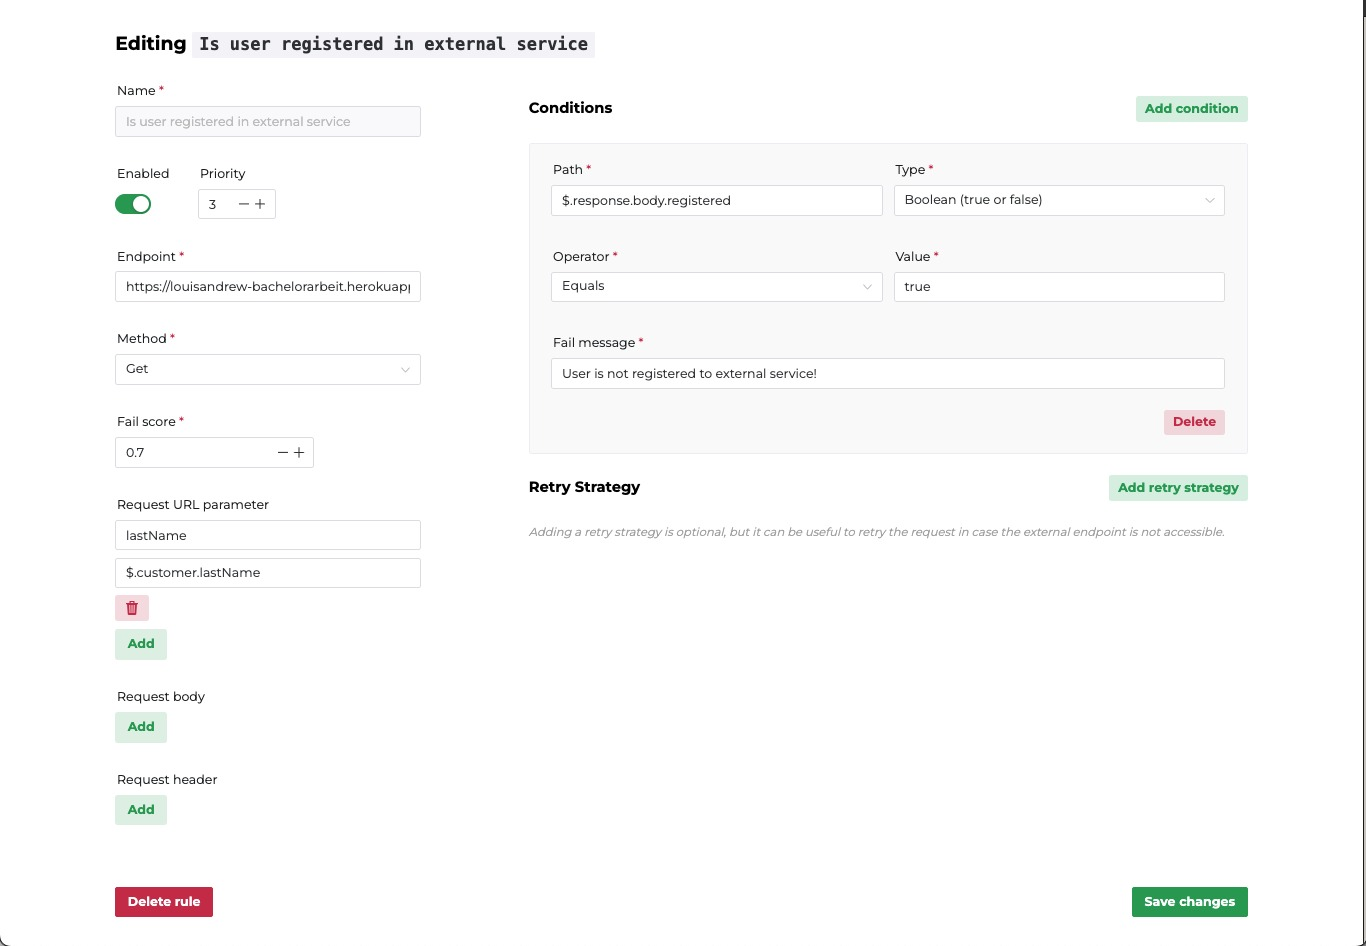
\includegraphics[width=\textwidth]{images/ss_sample_filled.jpeg}
      \caption{Screenshot of the rule management form}
    \end{figure}

    \subsubsection{Conditions Section}

      The \textsc{Conditions} section is a component, used to add one more condition to a validation rule. The \textsc{Conditions} section renders the list of conditions provided in a card, containing form fields for each attribute of the particular condition. Each card represents a single form, which also contains a form validation mechanism on its fields. 
      
      The available values for the \verb;operator; attribute of a condition depends on its \verb;type; attribute. To prevent an invalid condition being sent to the FDS, the \textsc{Operator} field is a select field, and its options are defined by the current value inputted on the \textsc{Type} field. The intention of the restriction is to make sure that the \verb;operator; chosen is always suitable with the corresponding \verb;type; attribute of the condition.

%       \begin{lstlisting}[style=es6, caption={Function to get list of available operators based on a condition's type attribute (TypeScript)}]
% const getAvailableOperators = (type: ConditionType) => {
%   switch (type) {
%     case "string":
%       return [
%         { label: "Equals", value: "eq" },
%         { label: "Starts with", value: "starts" },
%         { label: "Includes", value: "incl" },
%         { label: "Ends with", value: "ends" },
%       ]
%     case "number":
%       return [
%         { label: "Greater than", value: "gt" },
%         { label: "Greater than equals", value: "gte" },
%         { label: "Lesser than", value: "lt" },
%         { label: "Leser than equals", value: "lte" },
%         { label: "Equals", value: "eq" },
%       ]
%     case "array":
%       return [
%         { label: "Includes", value: "incl" },
%         { label: "Excludes", value: "excl" },
%         { label: "Number of items equals", value: "len" },
%         { label: "Is empty", value: "empty" },
%       ]
%     case "boolean":
%       return [{ label: "Equals", value: "eq" }]
%     default:
%       return []
%   }
% }
%       \end{lstlisting}

      \begin{figure}[!ht]
        \centering
        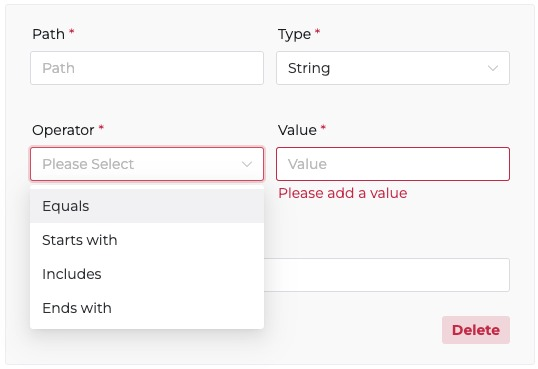
\includegraphics[width=0.8\textwidth]{images/ss_condition_op.jpeg}
        \caption{Screenshot of the "Operator" select field options, based on the current "Type" value}
      \end{figure}
      
      If more than one condition is provided, a radio field is also rendered, so that the user can choose one of the provided modifier for the list of conditions (either \textbf{\emph{ALL}} or \textbf{\emph{ANY}}). 

      An additional validation is implemented in the \textsc{Conditions} section. The validation not only make sure that all the required fields are filled, but also the value of the fields itself. For example, the validation will throw an error if the \textsc{Type} field is set to "Number", but the input value of the \textsc{Value} field is not a valid numerical value. 

    \subsubsection{Autocomplete Input}

      A JSONPath expression might be used as a value of some attributes within a \verb;ValidationRule; to access the runtime information during a validation process, such as the HTTP response from the external endpoint, runtime secrets or customer information. Unfortunately, it might be difficult to memorize the expressions needed to access certain values, and it might also confuse the user. 

      \begin{figure}[!ht]
        \centering
        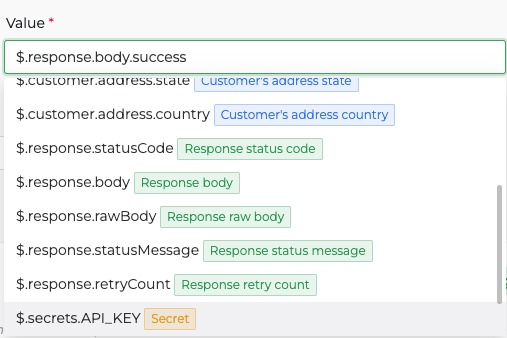
\includegraphics[width=0.5\textwidth]{images/ss_autocomplete.jpeg}
        \caption{Screenshot of the autocomplete input usage}
      \end{figure}

      To solve this problem, an autocomplete input field is provided in certain fields where a JSONPath expression is used. User can then display a list of possible JSONPath expressions by prefixing an input field with "\$", and choosing one of the expressions listed. User can also extend the expression chosen. The autocomplete input is used in the following form fields:

      \begin{itemize}
        \item \textsc{Path} field on \textsc{Conditions} section
        \item \textsc{Value} field on \textsc{Conditions} section
        \item Value field of a dynamic input\footnote{Autocompletion on \emph{\$.response} is only available on the \textsc{Conditions} section.}
      \end{itemize}

  \subsection{Validation Form}

    The validation form is a simple form similar to a customer registration form, specifically to mimic a new customer registration and to run a validation process directly after a new registration. Form validation is also implemented in the validation form to make sure that the customer information sent to the FDS is complete. A list of sample customers with specific characteristic is provided to pre-fill the validation form with a sample data. 

    \begin{figure}[!ht]
      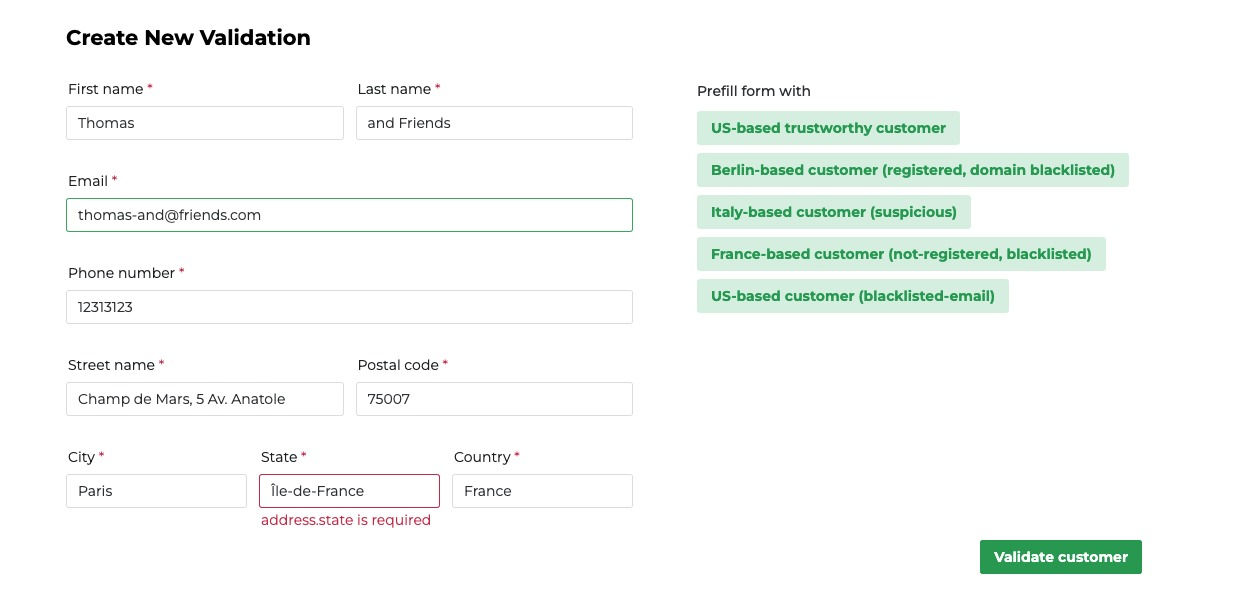
\includegraphics[width=\textwidth]{images/ss_customer_form.jpeg}
      \caption{Screenshot of the validation form}
    \end{figure}

    \newpage
    \begin{lstlisting}[style=es6, caption={Prefilling form values with a sample customer data (TypeScript)}]
const applySampleCustomer = (sampleCustomer: Customer) => {
  Object.assign(formValues, {
    ...sampleCustomer,
  })
}
\end{lstlisting}

    When the user filled the fields properly and clicked the \textsc{Validate customer} button, the UI sends an HTTP POST request to the FDS with the customer data as the payload to schedule a new validation process. As the FDS returns an ID of the validation process, the UI will then redirect the user to the validation progress page, showing the progress of the particular validation process in real time. 

    \begin{lstlisting}[style=es6, caption={Redirecting to the progress page when a validation process is scheduled successfully (TypeScript)}]
const { data } = await createNewValidation(customer)
if (data.validationId) {
  router.push(`/validations/${data.validationId}`)
}
\end{lstlisting}

  \subsection{Validation Progress}
  
    To receive the real time event stream sent by the FDS as described in \autoref{impl_sse}, the \verb;EventSource; API can be used on the client side. With the \verb;EventSource; API, a persistent connection to the FDS will be opened, and the messages sent will be received by the client in real time. Because the FDS sends the messages as a string in an event stream, the UI has to parse the message content into a valid JSON object before processing it. It is also important to close the connection to the event stream when it's no longer needed. The logic of closing the open connection when user leaves the current page is implemented on the UI. 

    \begin{lstlisting}[style=es6, caption={Using the EventSource API in the browser (TypeScript)}]
const source = new EventSource(url)

source.onmessage = messageEvent => {
  const data = JSON.parse(messageEvent.data)
}
\end{lstlisting}

    As the content of the message is parsed and identified as a valid \verb;ValidationResult; object, it is saved into the current state of the \verb;Validation; component, which renders the events of a validation process into a timeline component to give the user a better graphical overview of the current process. Vue3 uses the \emph{Proxy}\autocite[pp. 207-217]{gamma-1995} design pattern under the hood to establish a reactivity system on the UI, providing the possibility to update the timeline component every time a new validation result is published by the FDS. 

    The ID of the validation as well as the current fraud score are always displayed, to provide detailed information on the current validation process. Additionally, the customer data is also displayed as a JSON object, to give the user an insight on the customer data being sent to the FDS. 

    \begin{figure}[!ht]
      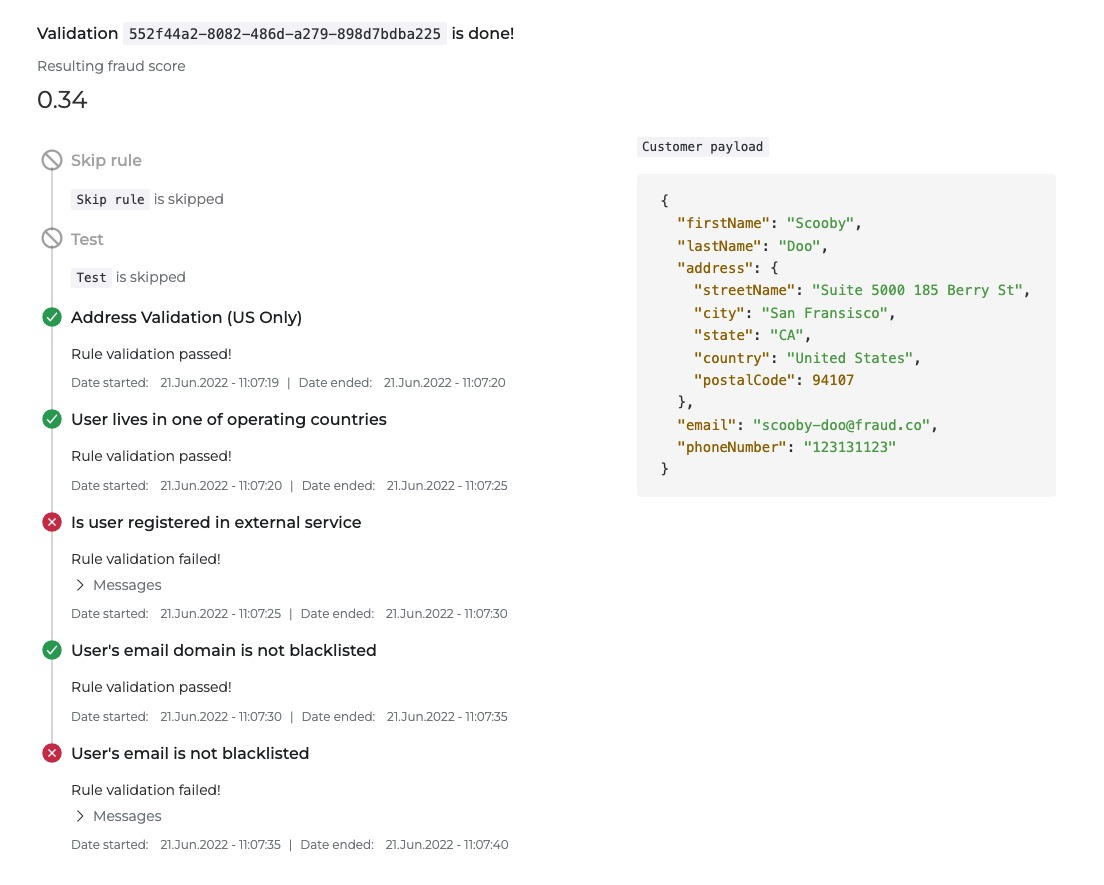
\includegraphics[width=\textwidth]{images/ss_validation_progress.jpeg}
      \caption{Screenshot of the validation progress in real time}
    \end{figure}
  
  \subsection{Runtime Secrets}

    A component to display a list of the available runtime secrets in a dialog is created. For security purposes, only the key of the secrets are displayed within the component. The component also provides a possibility to create a new runtime secret and to delete an existing secret. User can create a new secret by clicking on the \textsc{Create a new secret} button, and adding the essential information on the form fields displayed and delete an existing secret, a \textsc{Delete} button is displayed next to each secret's key name. When a user creates a new runtime secret or deletes an existing secret, the autocomplete options are changed according to the latest list of keys available in the database.

    \begin{figure}[!ht]
      \centering
      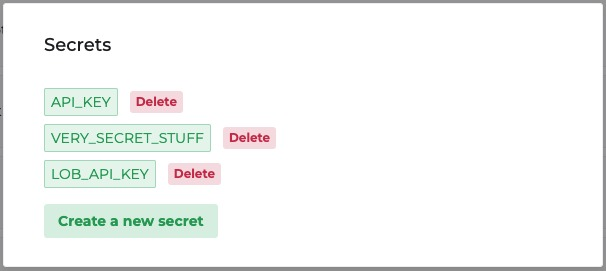
\includegraphics[width=0.8\textwidth]{images/ss_secrets.jpeg}
      \caption{Screenshot of a component to list available runtime secrets}
    \end{figure}
    
    
    